\documentclass[serif]{beamer}

\usetheme{CambridgeUS}
\usecolortheme{dolphin}

\usepackage{bm,color}
\usepackage{graphicx}
%\usepackage[brazil, english]{babel}
\usepackage{mathrsfs,amssymb,amsmath,enumerate}
%\usepackage{tgschola}
\usepackage{verbatim,graphicx,geometry,color}
\usepackage[utf8]{inputenc}
%\usepackage{setspace}
\usepackage{amsthm}

\newtheorem{prop}{Proposition}
%\newtheorem{lemma}{Lemma}[section]
\theoremstyle{definition}


\newcommand{\E}{\mathbb{E}}
\newcommand{\Var}{\mathrm{Var}}
\newcommand{\plim}{\overset{p}{\longrightarrow}}
\newcommand{\dlim}{\overset{d}{\longrightarrow}}

\usepackage{hyperref}
%\hypersetup{
%  colorlinks = true,
%  linkcolor = red!60!black,
%}
%\renewcommand{\thefootnote}{\arabic{footnote}}
%
%\makeatletter
%\let\@mycite\@cite
%\def\@cite#1#2{{\hypersetup{linkcolor=blue!60!black}[{#1\if@tempswa , #2\fi}]}}
%\makeatother


\begin{document}

\title[Quantitative Results]{Recombination Paper: Quantitative Results}
\author[A. Sollaci]{Alexandre Sollaci}
\institute[UChicago]{The university of Chicago}
\date{\today}

\begin{frame}[noframenumbering]
\titlepage
\end{frame}

\frame{ 
\title{Part I: Parameterization}
\author[]{}
\institute{}
\date{}
\titlepage
}

\frame{\frametitle{Introduction}
\begin{itemize}
\item To find the parameters I will present, I basically did a grid search.
\item Because the number of parameters is big, having fine grids and searching over every possible combination is not feasible.
\item Having this in mind, I first defined very coarse grids that spanned a large interval for each parameter. Having found the points that minimize the distance between the model and the data, I redefine finer grids around those points and search again. I did this 3 times.
\item Having said that, I found 2 parameterizations that yield vey similar results.
\end{itemize}
}

{\scriptsize{\frame{
\begin{table}[h!]
\caption{Model Parameters}
\centering
\begin{tabular}{ll}
\hline \hline
Parameter & Interpretation \\ \hline
$\eta^H$ & New technology quality increase. \\
$\eta^M$ & New combination quality increase. \\
$\eta^L$ & Reuse/refinement quality increase. \\
$\tau$ & Scale parameter of the new ideas distribution. \\
$\lambda$ & Scale parameter of the distribution of costs. \\
$\kappa$ & Shape parameter of the distribution of costs. \\
$\xi$ & Determines the fraction of viable combinations in a pool, $1/\xi$.\\
$\gamma$ & Determines the scale of the final goods production function. \\
$\epsilon$ & Determines the elasticity of intertemporal substitution of consumption.\\
$\beta$ & Intertemporal discount factor. \\
$I$ & Number of inventors.\\
$J$ & Number of firms.\\
\hline \hline
\end{tabular}
\end{table}
}}}

\frame{
\begin{table}[h!]
\caption{Parameters that do not affect patent type distribution.}
\centering
\begin{tabular}{lp{3cm}p{5cm}}
\hline \hline
variable & value & Moment \\ \hline
$\eta^L$ & 0 & Normalized. \\
$\gamma$ & 0.6 & Fits the labor share of GDP \\
$\epsilon$ & 2 & Taken from Acemoglu, Akcigit, Bloom and Kerr (2013). \\
$\beta$ & 0.954 & $=\frac{1}{1+r}$, with $r = 5\%$. \\
$J$ & depends on parameterization & chosen to fit average growth rate. \\
\hline \hline
\end{tabular}
\end{table}
}

\frame{\frametitle{Moments of the Patent Type Distribution}
\begin{itemize}
\item I used 10 moments to find the rest of the parameters:
\begin{itemize}
\item New technology and new combination fractions in 1850, 1900, 1950 and 2000 (8 moments);
\item Reuse fraction peak value and year that it reaches the peak. 
\end{itemize}
\end{itemize}
}

\frame{\frametitle{Parameterization 1: does not include $I$ as a parameter}
\begin{table}[h!]
\caption{Parameters related to the patent type distribution.}
\centering
\begin{tabular}{ll}
\hline \hline
Parameter & Value \\ \hline
$\eta^H$ & 0.2 \\
$\eta^M$ & 0.04 \\
$\tau$ & 400 \\
$\lambda $ & 2.1 \\
$\kappa$ & 7 \\
$\xi$ & 75 \\
\hline \hline
\end{tabular}
\end{table}
and 
\[ I = 500; \qquad J = 910 \]
}

\frame{
\centering
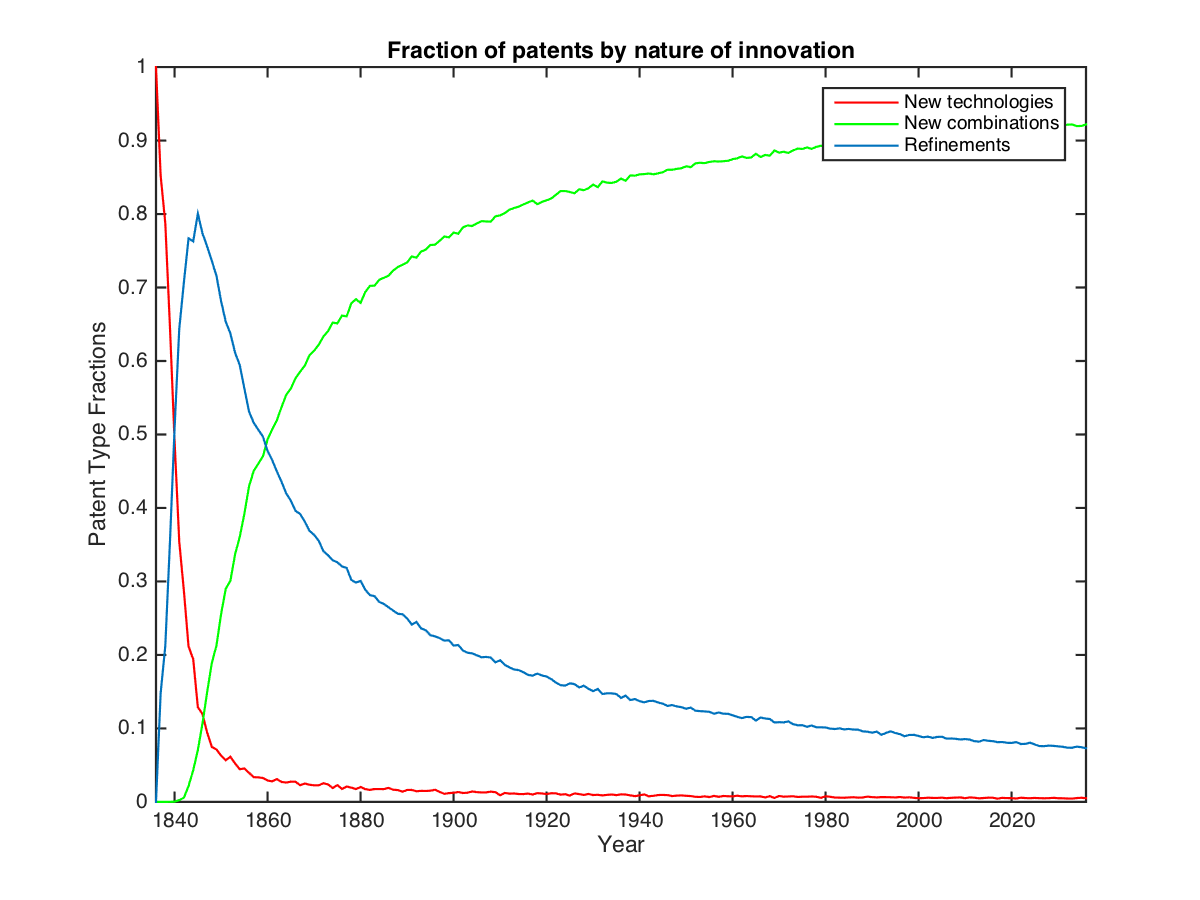
\includegraphics[scale=.6]{patents1.png}
}

\frame{
\centering
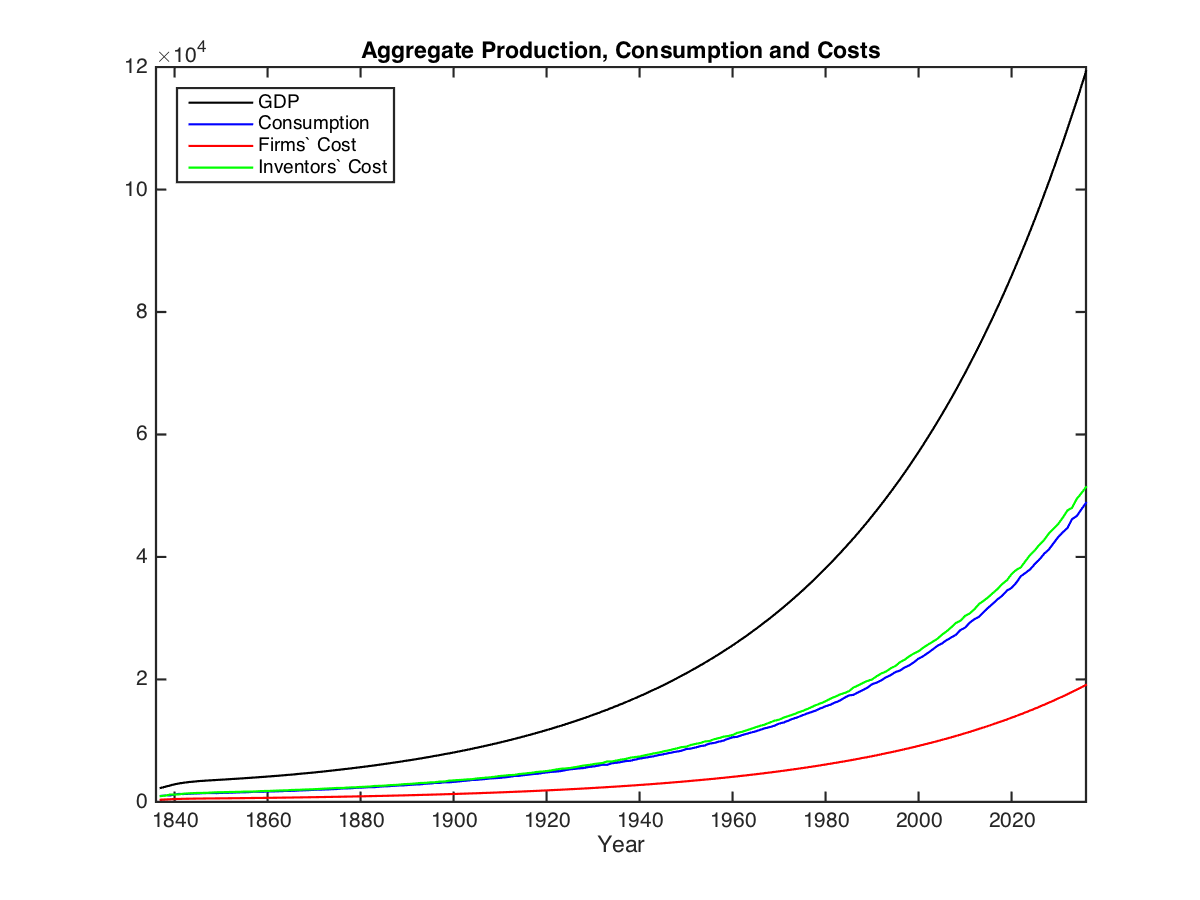
\includegraphics[scale=.6]{aggregates1.png}
}

\frame{\frametitle{Parameterization 2: includes $I$ as a parameter}
\begin{table}[h!]
\caption{Parameters related to the patent type distribution.}
\centering
\begin{tabular}{ll}
\hline \hline
Parameter & Value \\ \hline
$\eta^H$ & 0.2 \\
$\eta^M$ & 0.05 \\
$\tau$ & 800 \\
$\lambda $ & 2 \\
$\kappa$ & 7 \\
$\xi$ & 150 \\
$I$ & 800 \\
\hline \hline
\end{tabular}
\end{table}
and 
\[  J = 1750 \]
\begin{itemize}
\item I will use this version to compute the counterfactuals.
\end{itemize}
}

\frame{
\centering
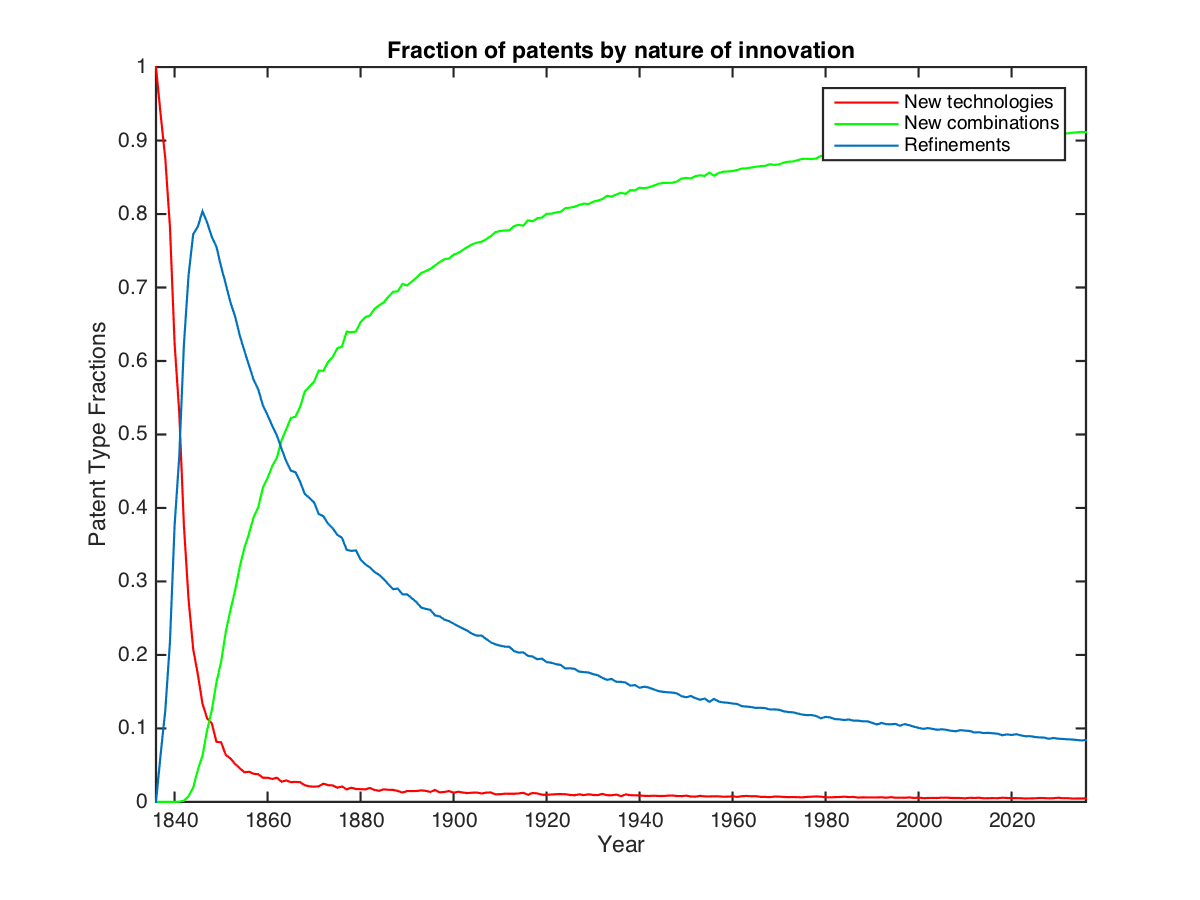
\includegraphics[scale=.6]{patents2.png}
}

\frame{
\centering
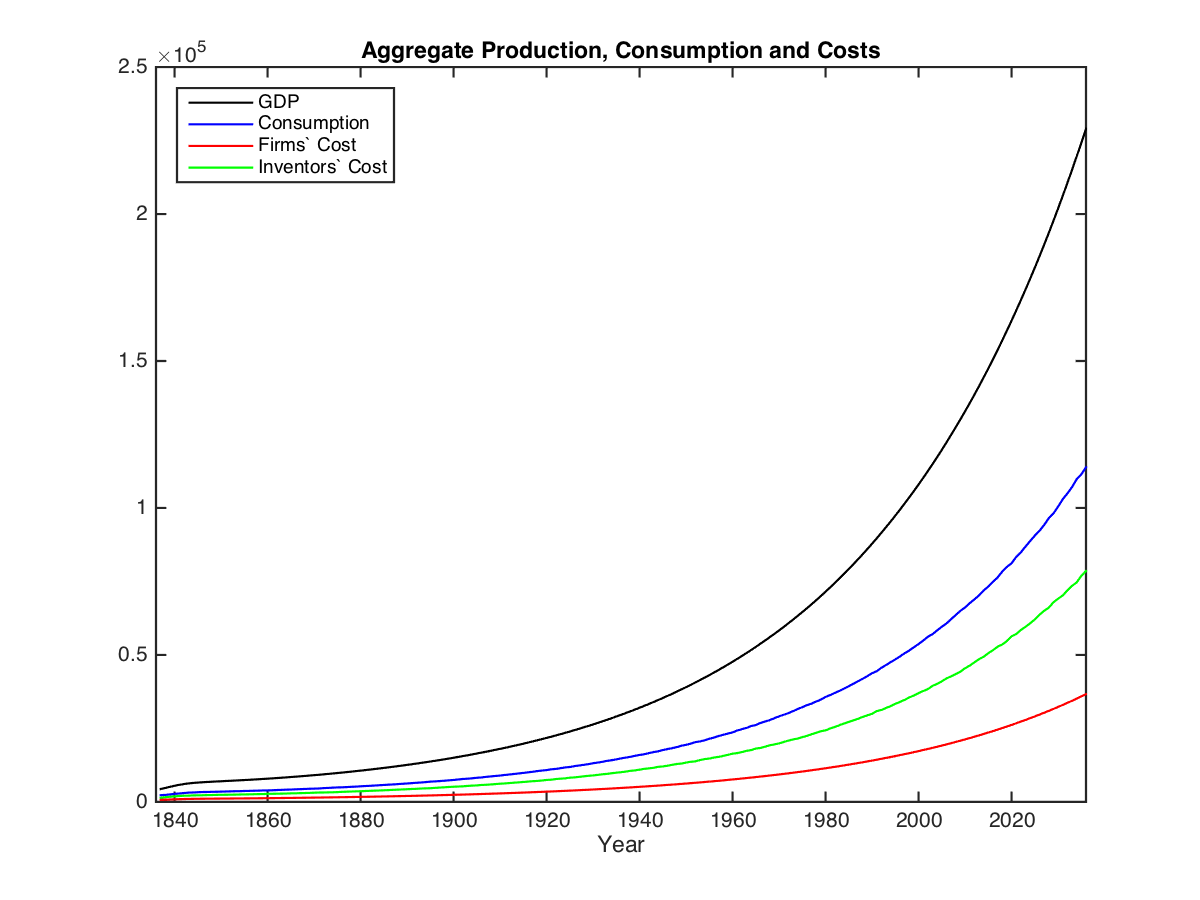
\includegraphics[scale=.6]{aggregates2.png}
}

\frame{ 
\title{Part II: Counterfactuals}
\author[]{}
\institute{}
\date{}
\titlepage
}

\frame{\frametitle{Introduction}
\begin{itemize}
\item The counterfactual here is a subsidy on patent creation. 
\item I will consider a subsidy for new technology patents only, new combination patents only and both. 
\item I will also alter the duration of the subsidy, lasting for 50 or 100 years.
\end{itemize}
}

\section{25\% subsidy on new technologies for 50 years}

\frame{
\centering
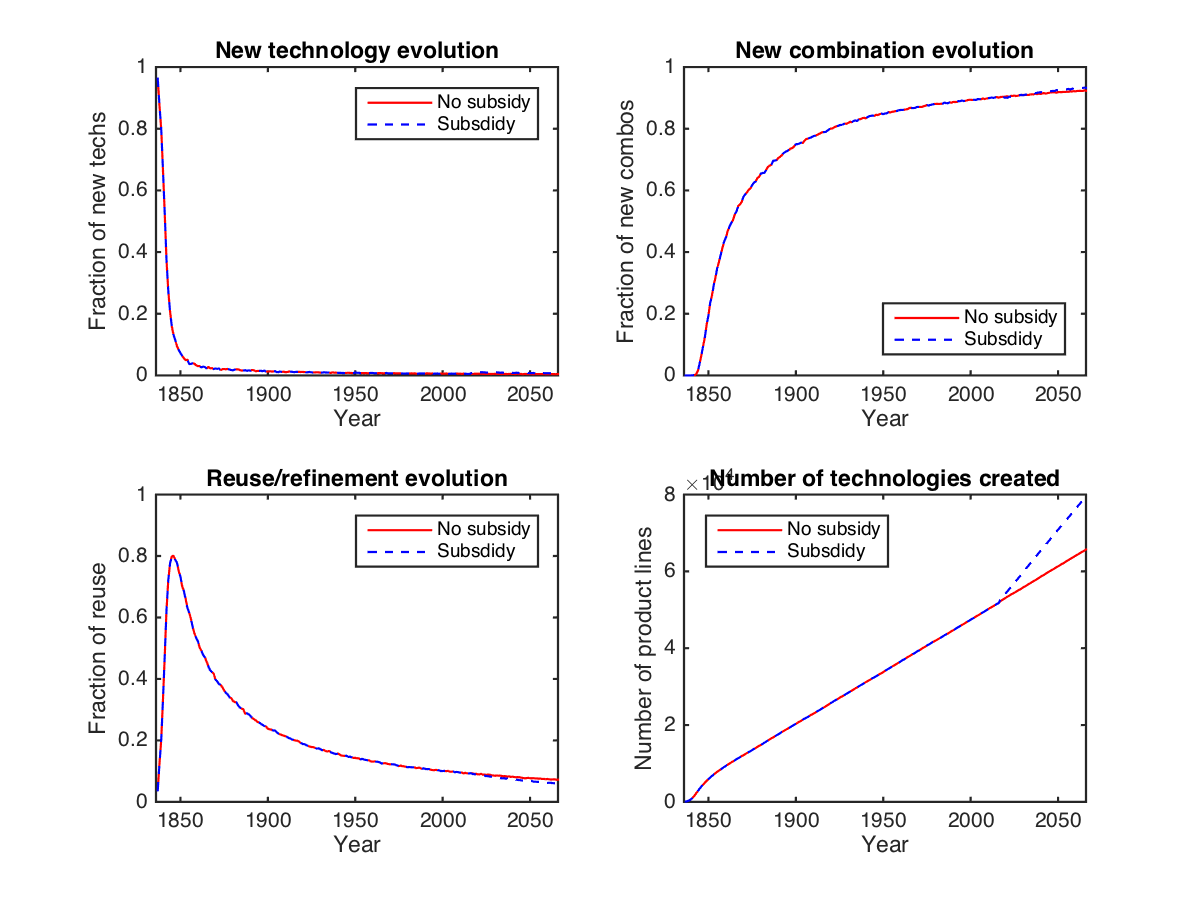
\includegraphics[scale=.6]{counterfactual/patentsNT_25pp_50y.png}
}

\frame{
\centering
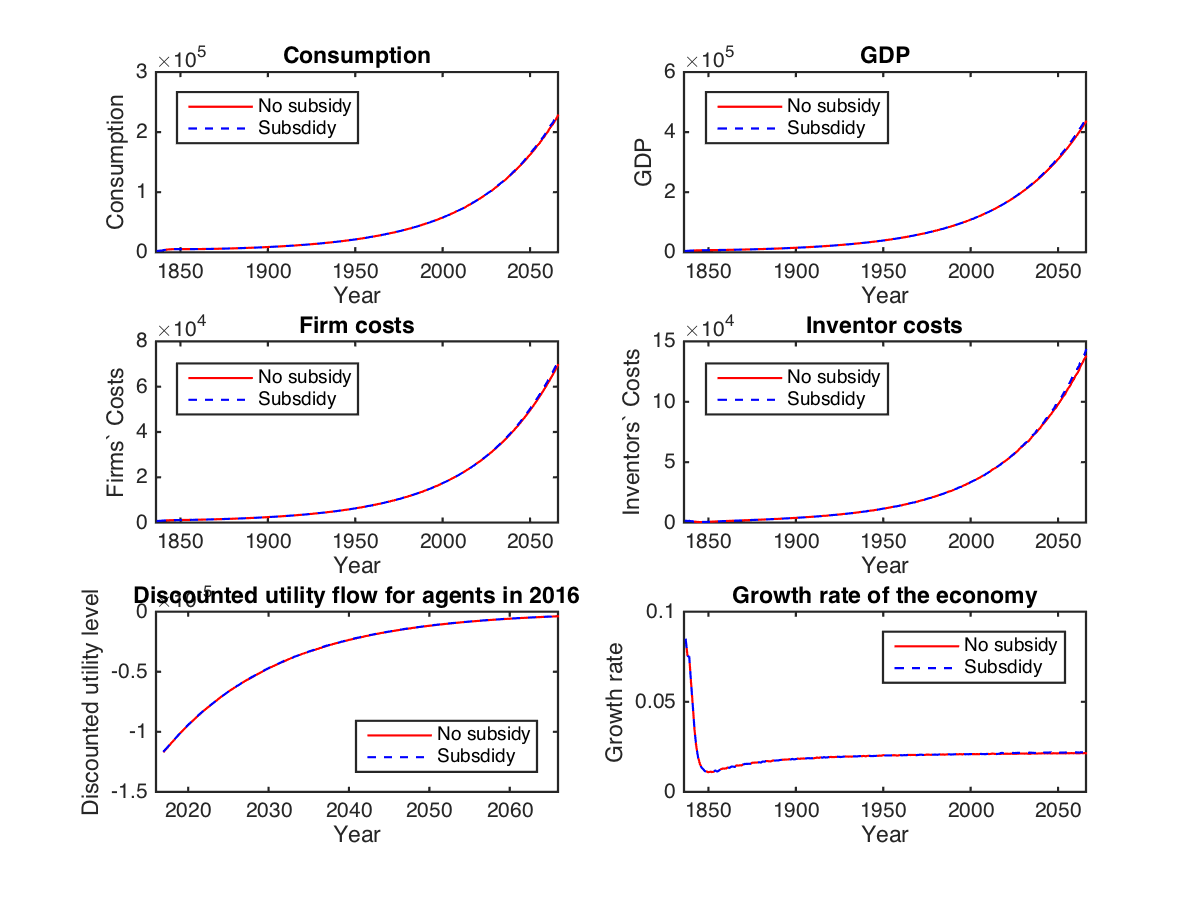
\includegraphics[scale=.6]{counterfactual/aggregatesNT_25pp_50y.png}
}

\frame{
\begin{table}
\begin{tabular}{|l|l|l|l|}
\hline
&\textbf{Subsidy}&\textbf{No subsidy}&\textbf{\% Change}\\\hline
\textbf{Welfare}&-0.00016789&-0.00016727&0.0036889\\\hline
\textbf{\# technologies}&65679&79604&0.21202\\\hline
\textbf{Average GDP growth}&0.021321&0.021753&0.020279\\\hline
\end{tabular}

\end{table}
}

\section{25\% subsidy on new technologies for 100 years}

\frame{
\centering
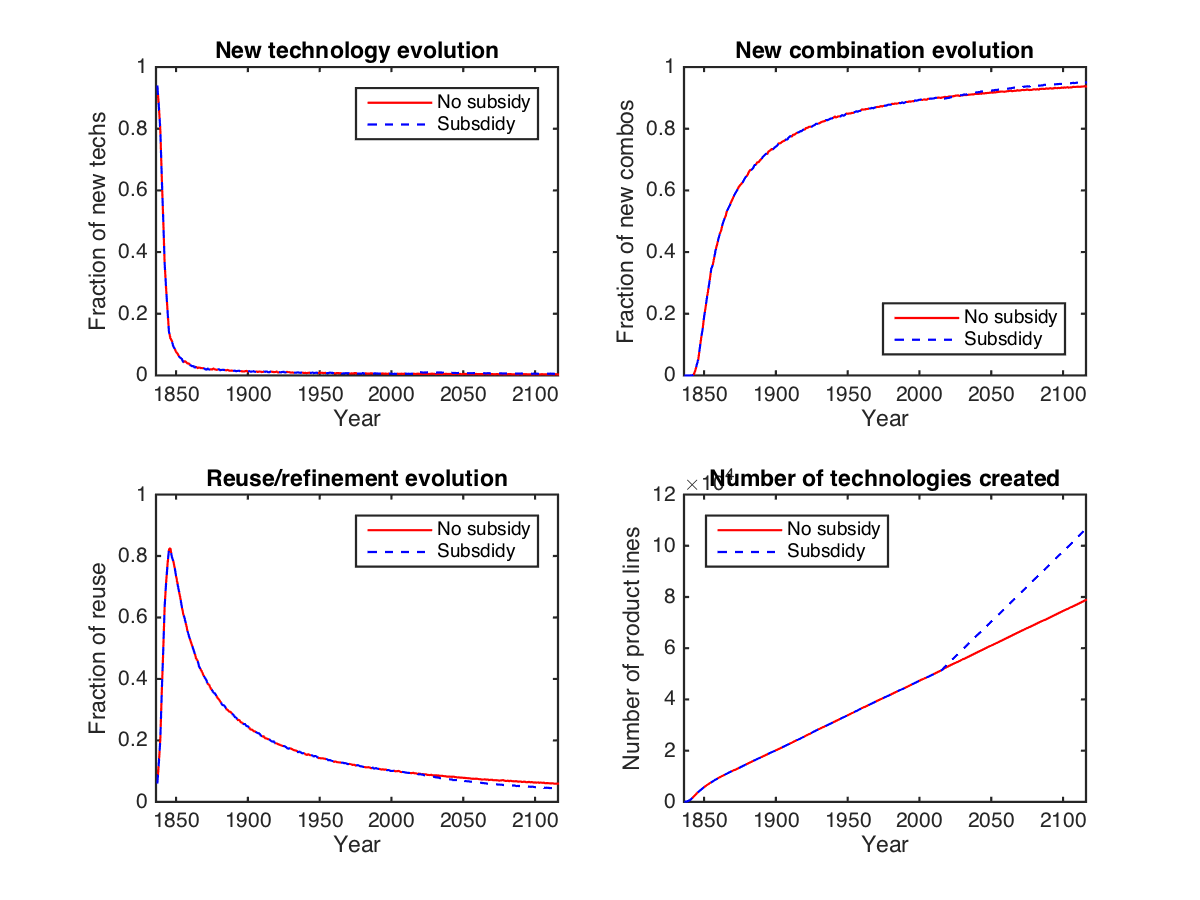
\includegraphics[scale=.6]{counterfactual/patentsNT_25pp_100y.png}
}

\frame{
\centering
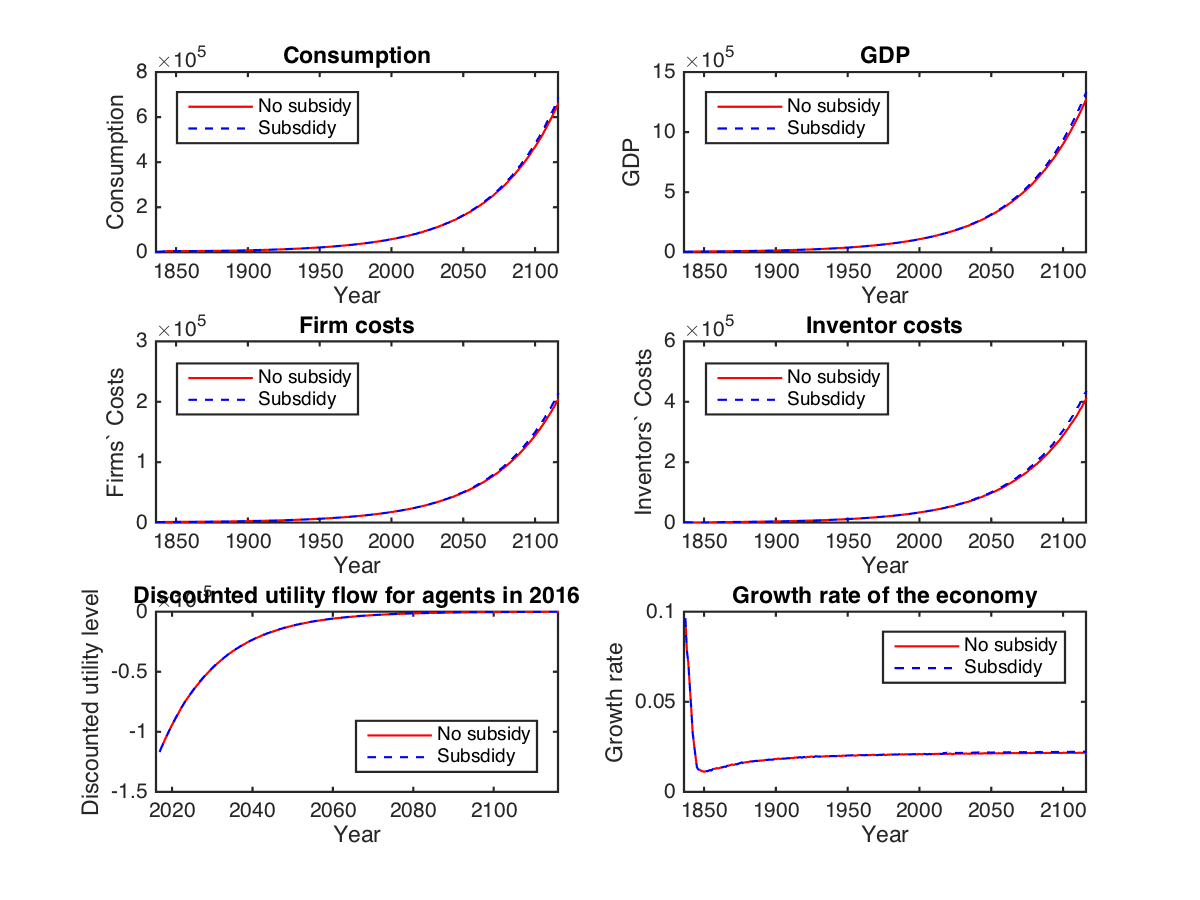
\includegraphics[scale=.6]{counterfactual/aggregatesNT_25pp_100y.png}
}

\frame{
\begin{table}
\begin{tabular}{|l|l|l|l|}
\hline
&\textbf{Subsidy}&\textbf{No subsidy}&\textbf{\% Change}\\\hline
\textbf{Welfare}&-0.00017249&-0.00017185&0.0036683\\\hline
\textbf{\# technologies}&78806&106595&0.35263\\\hline
\textbf{Average GDP growth}&0.021463&0.021933&0.021896\\\hline
\end{tabular}

\end{table}
}

\section{25\% subsidy for new combinations for 50 years}

\frame{
\centering
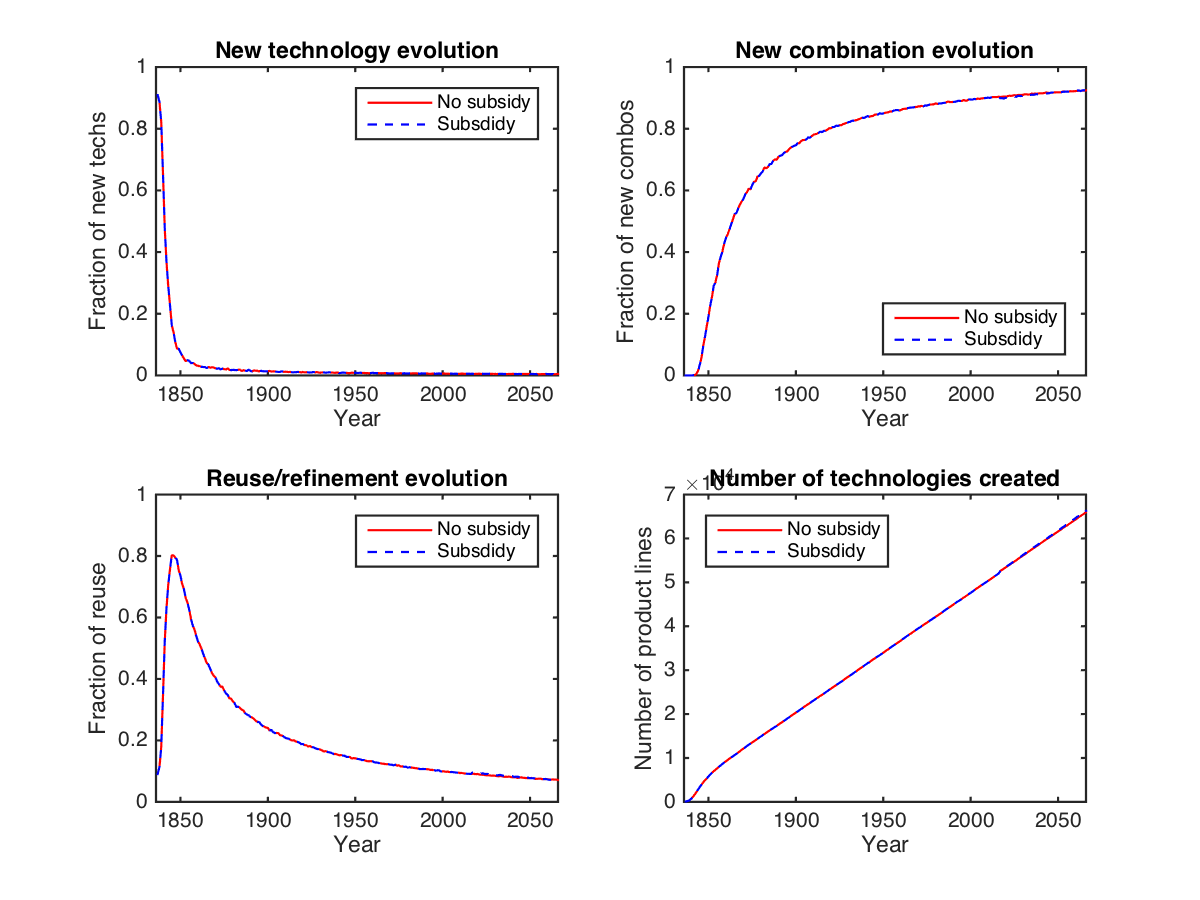
\includegraphics[scale=.6]{counterfactual/patentsNC_25pp_50y.png}
}

\frame{
\centering
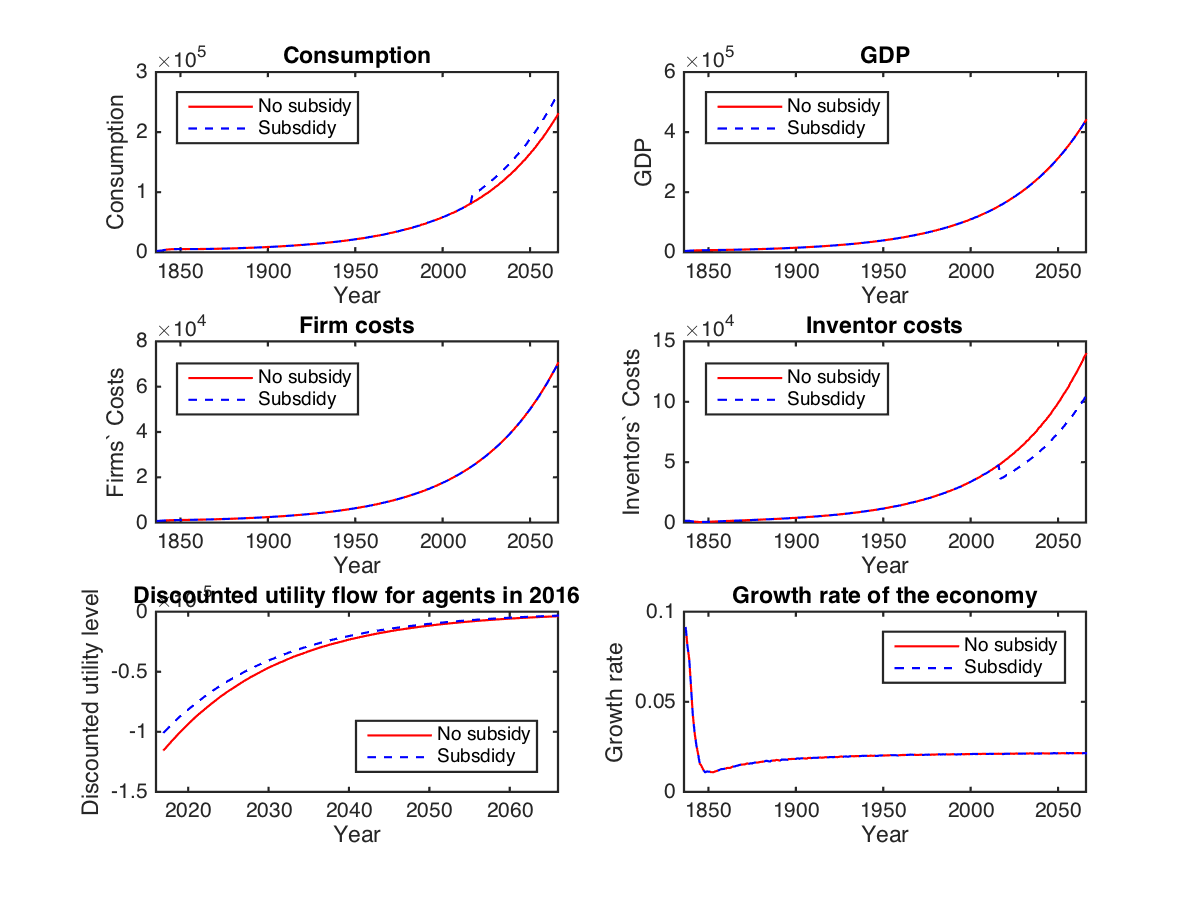
\includegraphics[scale=.6]{counterfactual/aggregatesNC_25pp_50y.png}
}

\frame{
\begin{table}
\begin{tabular}{|l|l|l|l|}
\hline
&\textbf{Subsidy}&\textbf{No subsidy}&\textbf{\% Change}\\\hline
\textbf{Welfare}&-0.00016624&-0.0001447&0.12958\\\hline
\textbf{\# technologies}&65968&66259&0.0044112\\\hline
\textbf{Average GDP growth}&0.021339&0.021305&-0.0015829\\\hline
\end{tabular}

\end{table}
}

\section{25\% subsidy on new combinations for 100 years}

\frame{
\centering
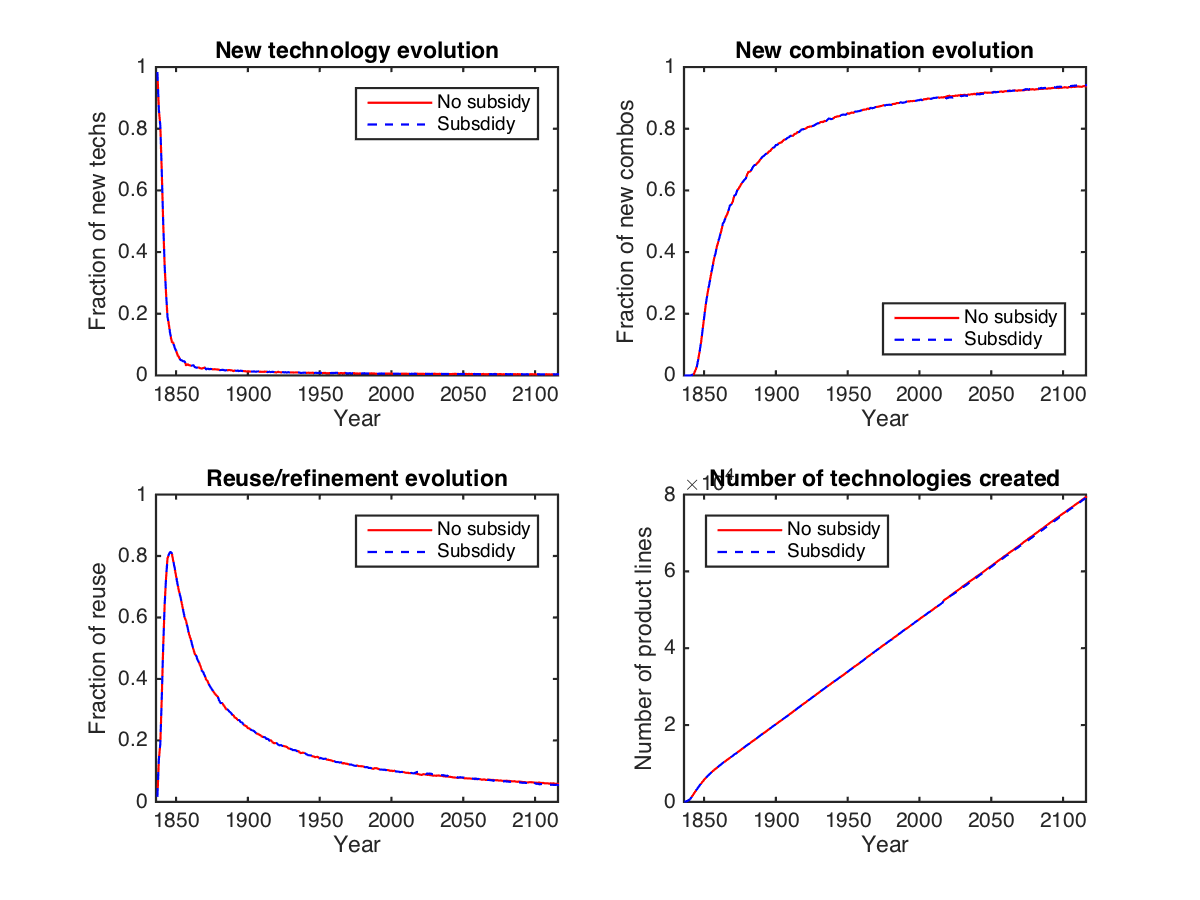
\includegraphics[scale=.6]{counterfactual/patentsNC_25pp_100y.png}
}

\frame{
\centering
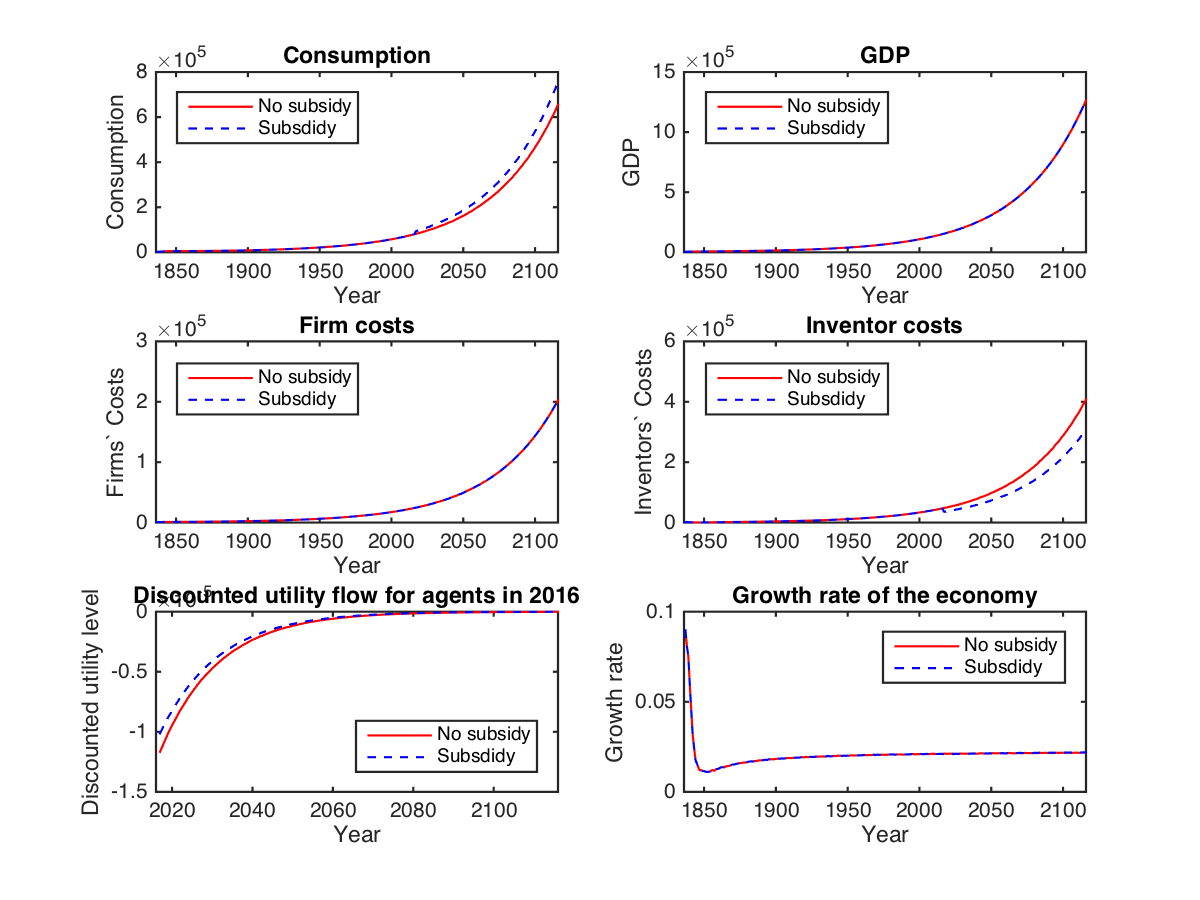
\includegraphics[scale=.6]{counterfactual/aggregatesNC_25pp_100y.png}
}

\frame{
\begin{table}
\begin{tabular}{|l|l|l|l|}
\hline
&\textbf{Subsidy}&\textbf{No subsidy}&\textbf{\% Change}\\\hline
\textbf{Welfare}&-0.00017332&-0.00015093&0.12921\\\hline
\textbf{\# technologies}&79361&79179&-0.0022933\\\hline
\textbf{Average GDP growth}&0.021469&0.02149&0.00099304\\\hline
\end{tabular}

\end{table}
}

\section{25\% subsidy for all patents for 50 years}

\frame{
\centering
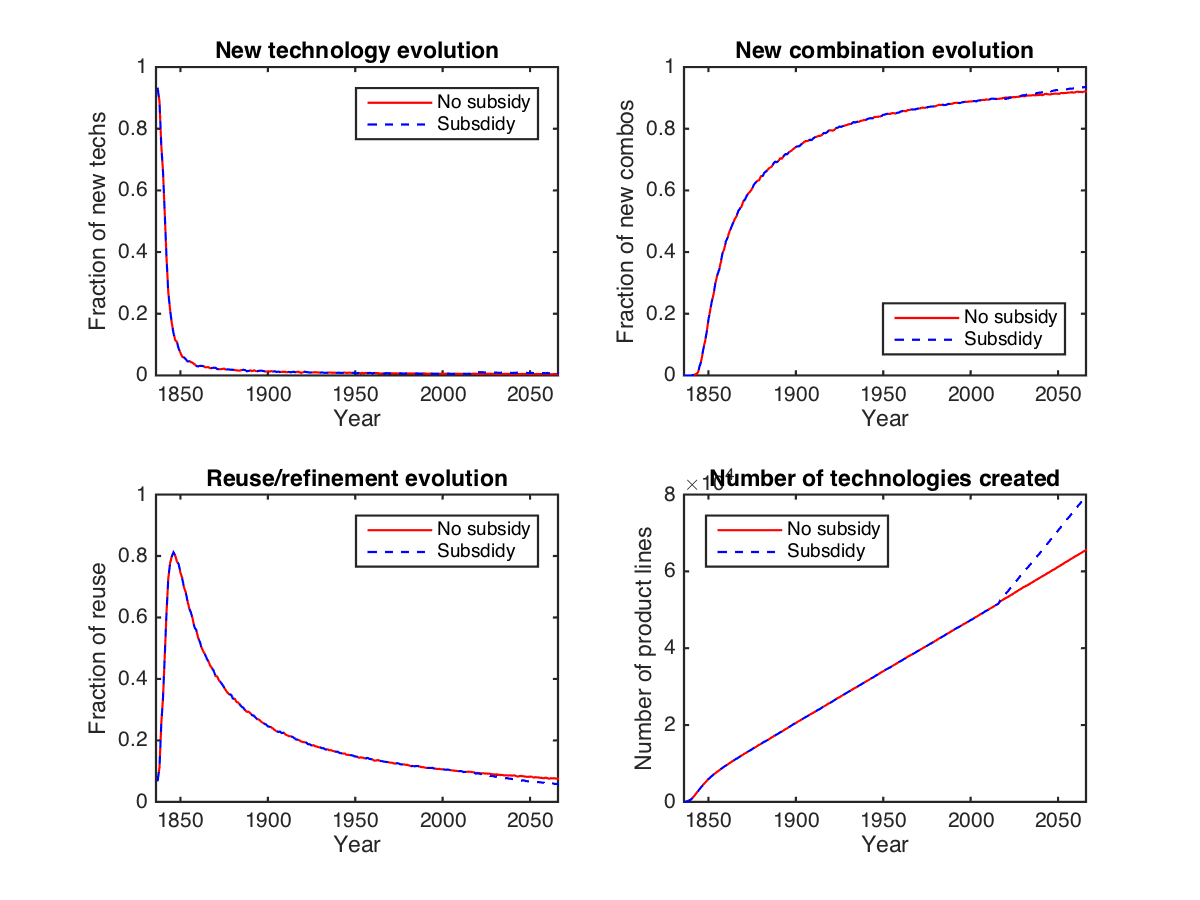
\includegraphics[scale=.6]{counterfactual/patentsALL_25pp_50y.png}
}

\frame{
\centering
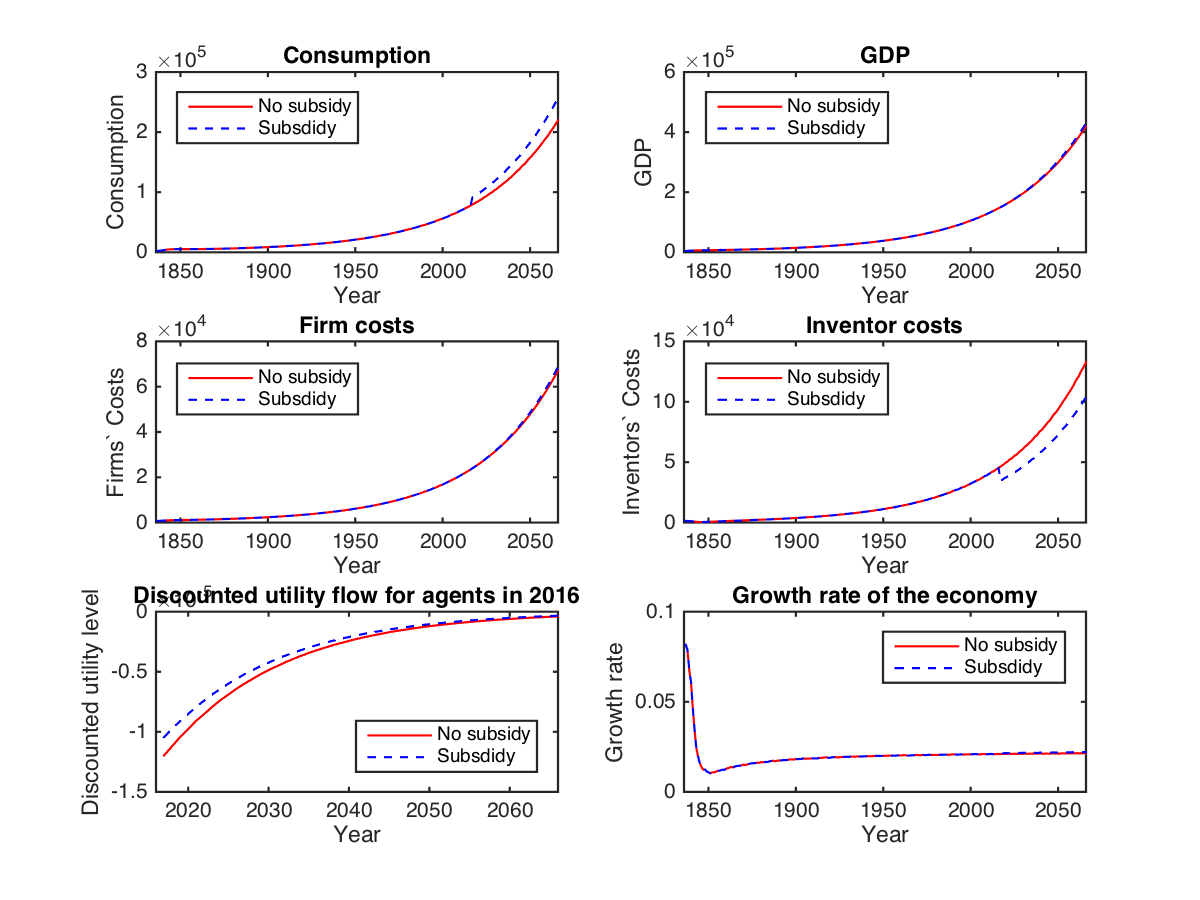
\includegraphics[scale=.6]{counterfactual/aggregatesALL_25pp_50y.png}
}

\frame{
\begin{table}
\begin{tabular}{|l|l|l|l|}
\hline
&\textbf{Subsidy}&\textbf{No subsidy}&\textbf{\% Change}\\\hline
\textbf{Welfare}&-0.00017333&-0.00015062&0.13101\\\hline
\textbf{\# technologies}&65551&79535&0.21333\\\hline
\textbf{Average GDP growth}&0.021245&0.02175&0.02379\\\hline
\end{tabular}

\end{table}
}

\section{25\% subsidy for all patents for 100 years}

\frame{
\centering
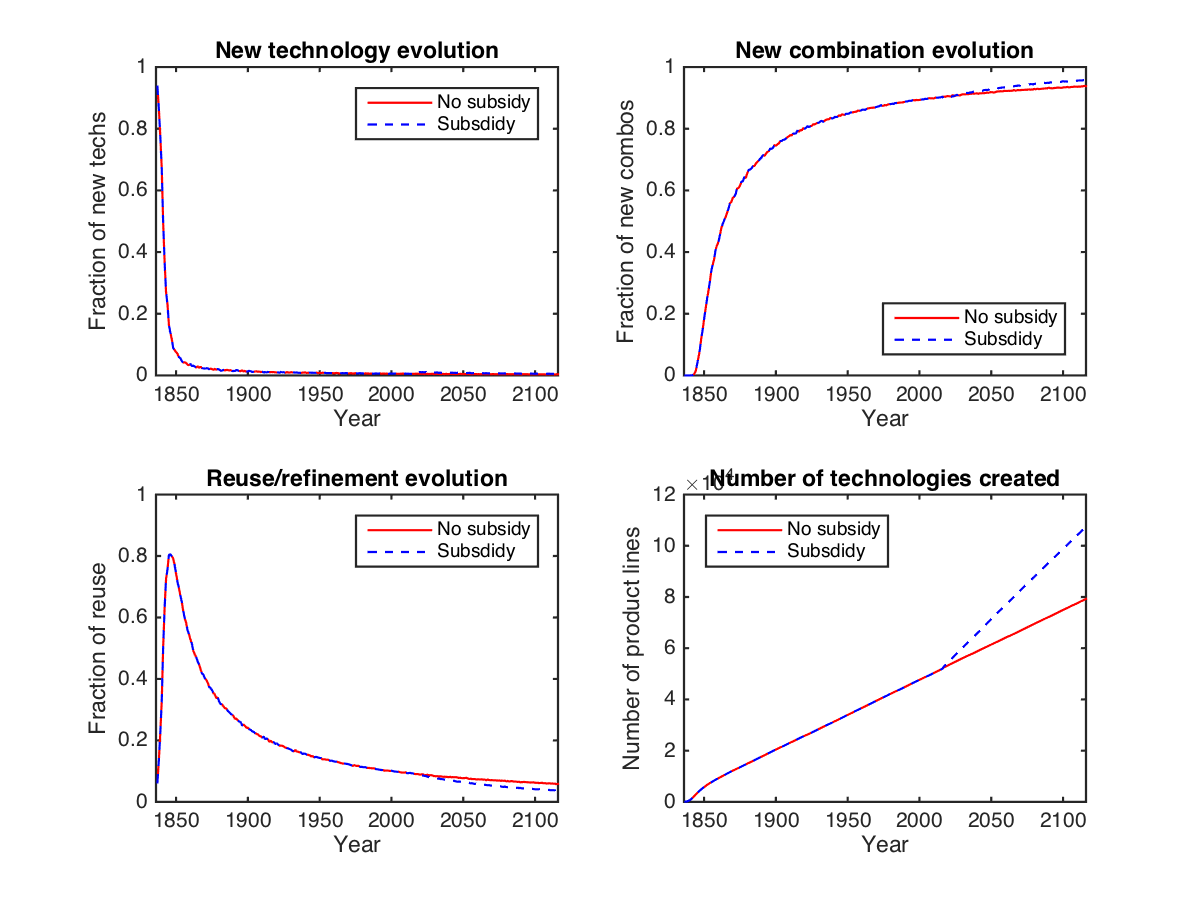
\includegraphics[scale=.6]{counterfactual/patentsALL_25pp_100y.png}
}

\frame{
\centering
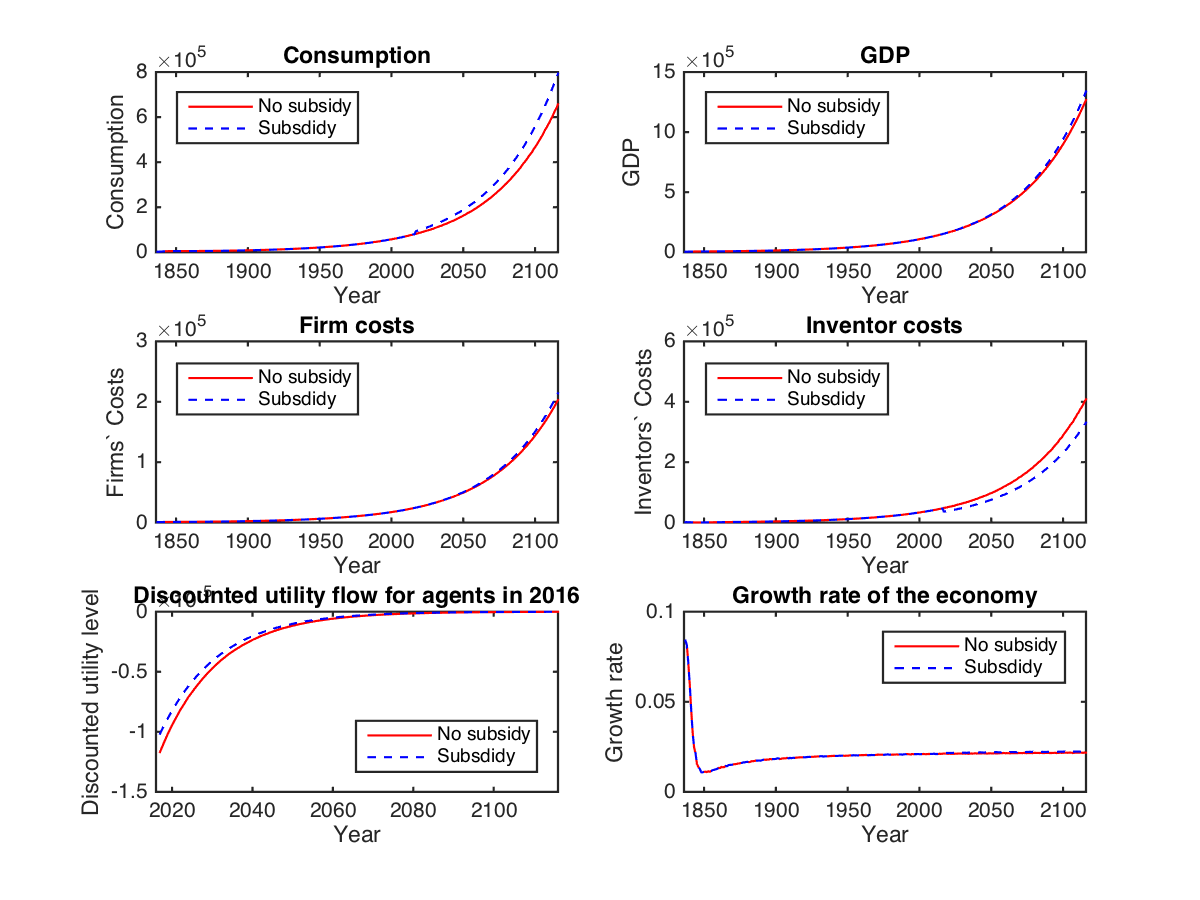
\includegraphics[scale=.6]{counterfactual/aggregatesALL_25pp_100y.png}
}

\frame{
\begin{table}
\begin{tabular}{|l|l|l|l|}
\hline
&\textbf{Subsidy}&\textbf{No subsidy}&\textbf{\% Change}\\\hline
\textbf{Welfare}&-0.00017313&-0.00015022&0.13232\\\hline
\textbf{\# technologies}&79265&107507&0.3563\\\hline
\textbf{Average GDP growth}&0.021484&0.022047&0.0262\\\hline
\end{tabular}

\end{table}
}

\frame{\frametitle{Patterns}
\begin{itemize}
\item The pattern is clear: subsidizing new combinations will have no effect no patent shares or in the number of technologies, but it will have the highest effect on welfare.

\item In fact, growth is even smaller when subsidizing new combinations, since inventors might revert from producing new technologies to produce new combinations. But the number of combination possibilities is so great that new combinations more than make up for the difference.

\item Finally, subsidizing new combinations and new technologies at the same time has a bigger effect than the sum of the two subsidies alone. There is a complementarity between the two as new technologies always create more hot product lines.

\item Finally, we can experiment with different subsidies. For fun, the following has 10\% subsidy for new technologies and 50\% subsidy for new combinations. This subsidy runs for 100 years.
\end{itemize}
}

\section{10\% new technology, 50\% new combination, 100 years}

\frame{
\centering
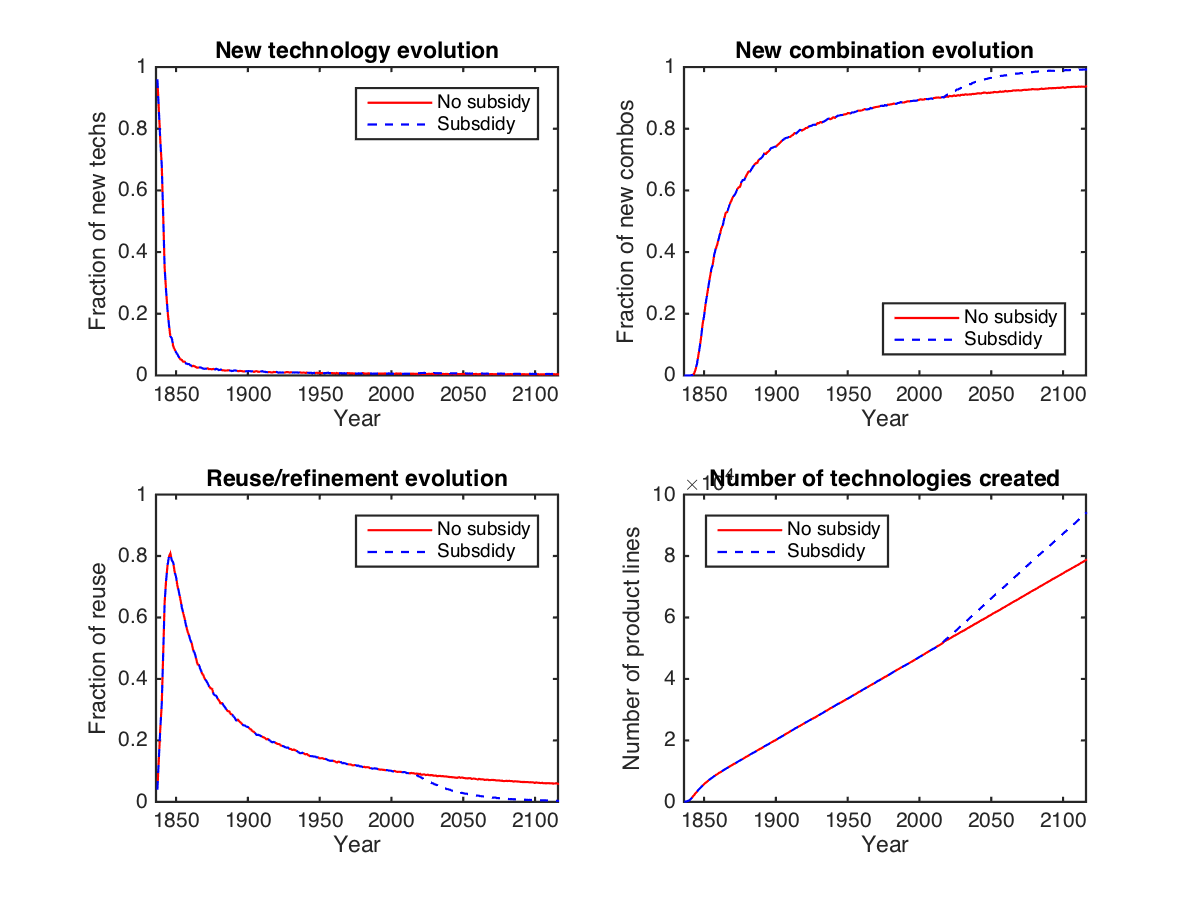
\includegraphics[scale=.6]{counterfactual/patentsALL_10-50pp_100y.png}
}

\frame{
\centering
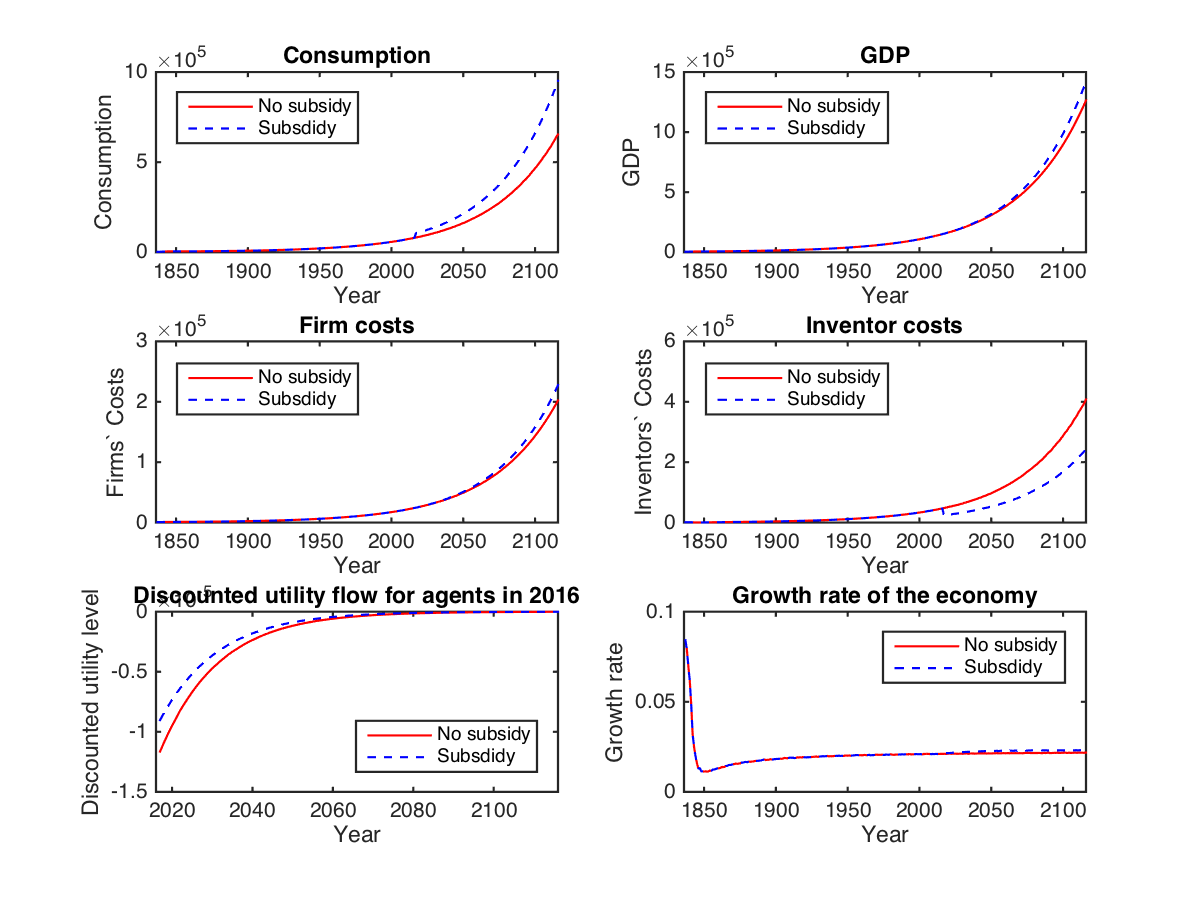
\includegraphics[scale=.6]{counterfactual/aggregatesALL_10-50pp_100y.png}
}

\frame{
\begin{table}
\begin{tabular}{|l|l|l|l|}
\hline
&\textbf{Subsidy}&\textbf{No subsidy}&\textbf{\% Change}\\\hline
\textbf{Welfare}&-0.00017347&-0.00013343&0.23086\\\hline
\textbf{\# technologies}&78682&93980&0.19443\\\hline
\textbf{Average GDP growth}&0.021469&0.022677&0.056245\\\hline
\end{tabular}

\end{table}
}



\end{document}